\chapter{0D LSP Model} \label{chp:models}

    To correctly predict the temperature increase of the gas that should be expected when laser energy is input, the heat capacity of argon and hydrogen was modelled. 
    
    Argon is the current gas used in experiments, as it is economical and easy to ionize. Hydrogen is projected to be used in the full-scale LTP engine for its increased $I_\mathrm{sp}$ due to having lower molecular weight.

    \section{Equilibrium calculations} \label{sec:equilibrium calcs}
        
        The following seventh order polynomials and their coefficients ($a_1$ to $a_7$, $b_1$, and $b_2$), from \textcite{mcbrideNASAGlennCoefficients2002}, were implemented in Python. Species of interest were \ce{H}, \ce{H2}, \ce{Ar}, \ce{Ar+}, and electrons \ce{e-}. Plasma temperatures studied allowed us to treat the argon as singly ionized, and the hydrogen as dissociated. The heat capacity at constant pressure, as well as the temperature ($T$) dependent part of enthalpy and entropy of each species are given by $C_p^0$, $H^0$ and $S^0$, respectively. $\bar R$ is the universal gas constant.

        \begin{equation}
            C_p^0 (T)/\bar R = a_1 T^{-2} + a_2 T^{-1} + a_3 + a_4   T + a_5 T^2 + a_6 T^3 + a_7 T^4
        \end{equation} 
        
        \begin{equation}
            H^0 (T)/\bar RT = -a_1 T^{-2} + a_2 \ln(T)/T + a_3 + a_4 T / 2 + a_5 {T^2}/3 + a_6 {T^3}/4 + a_7 {T^4}/5 + b_1/T
        \end{equation}
        
        \begin{equation}
            S^0(T)/\bar R = -a_1 T^{-2}/2 - a_2 T^{-1} + a_3\ln(T) + a_4   T + a_5 {T^2}/2 + a_6 T^3/3 + a_7 T^4/4 + b_2
        \end{equation}

        Next, the functions for entropy $\bar s_i$ of each species $i$ and Gibbs energy $\bar g_i$, both per \unit{kmol}, were implemented. These values depend on temperature $T$ and partial pressure $p_i$. $y_i$ is the molar fraction of the species, and $p_{ref}$ is the reference pressure, equal to \qty{1}{bar}.
        
        \begin{equation}
            \bar s_i (T, p_i) = \bar s_i^0 (T) - \bar R \ln \frac{y_i p}{p_{ref}}
        \end{equation}

        \begin{equation}
            \bar g_i = \bar h_i - T \bar s_i
        \end{equation}

        Considering the number of moles $n_i$, expressions of the Gibbs energy of the two mixtures $G_{mixture}$ are found:

        Starting with \qty{1}{kmol} argon,
        \begin{equation}
            G_{mixture,\: Ar}(T, p) = n_{Ar} \bar g_{Ar}(T, p_{Ar}) + n_{Ar+} \bar g_{Ar+}(T, p_{Ar+}) + n_e \bar g_e(T, p_e)
        \end{equation}

        Starting with \qty{1}{kmol} hydrogen,
        \begin{equation}
            G_{mixture,\: H_2}(T, p) = n_H \bar g_H(T, p_H) + n_{H2} \bar g_{H2}(T, p_{H2})
        \end{equation}

        \autoref{fig:Gibbs} plots the Gibbs energy of the hydrogen mixture as a function of its degree of dissociation $x$, for different total pressures $p$.

        \begin{figure}[!ht]
            \centering
            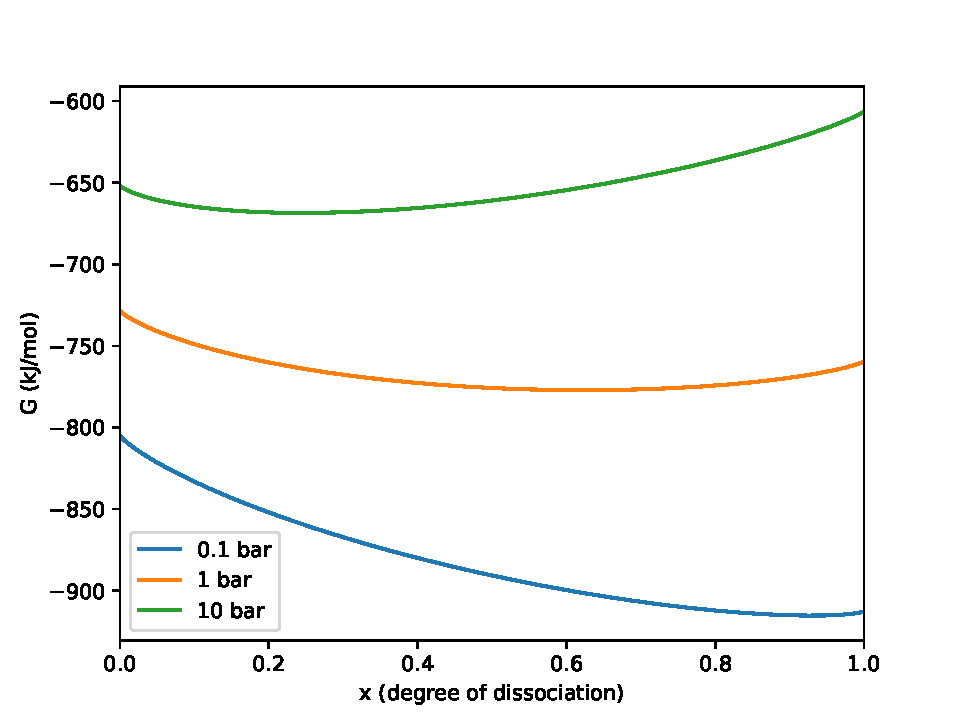
\includegraphics[width=0.7\textwidth]{assets/2 models/Gibbs.pdf}
            \caption{Gibbs free energy (G) plotted against the degree of dissociation (x) of hydrogen under three different pressures}
            \label{fig:Gibbs}
        \end{figure}

        A similar dissociation graph can be found with argon, but with three species. The Gibbs energy is then minimized to determine the molar fractions $y_i$ at which the mixture reaches equilibrium. From this, the enthalpy $H$ of the mixture was found. The $C_p$ of the mixture was then calculated from the enthalpy with:

        \begin{equation}
            C_p = \frac{\partial H}{\partial T}
        \end{equation}
        
        For argon, these calculated $C_p$ values were validated against values from CEA \cite{CEARUNRev4} in \autoref{fig:Cp_compare}.
        
        \begin{figure}[!ht]
            \centering
            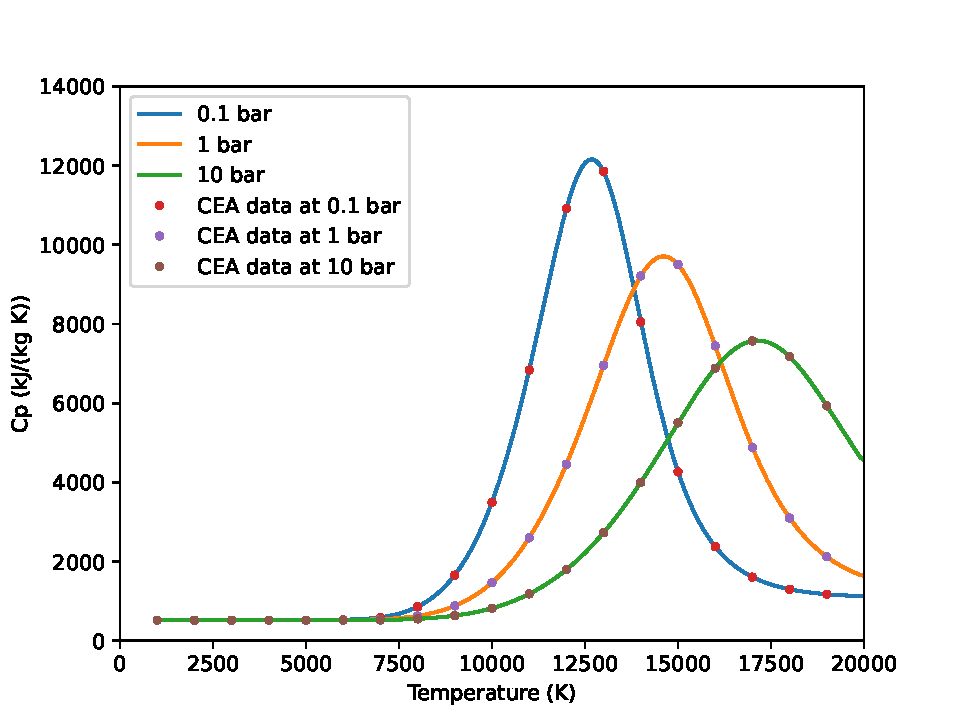
\includegraphics[width=0.7\textwidth]{assets/2 models/Cp_compare.pdf}
            \caption{Comparing calculated $C_p$ values of argon to those from CEA}
            \label{fig:Cp_compare}
        \end{figure}
    
    \section{Bremsstrahlung}
        
        The main source of radiation found in LSP is Bremsstrahlung, or braking radiation. When an electron's velocity vector changes around a heavier ion (elastic collision), a photon is released \todo{change this explanation}. The total radiated power can then be calculated with the formulas presented in the following table.

        \todo{Brems formula table} \textcite{glasstoneControlledThermonuclearReactions1975}

        The first relation was used for the remainder of the calculations. 

        There is also a question regarding whether the plasma is a surface emitter or a volume emitter. This is determined by calculating the plasma frequency at a typical electron density and comparing it to the wavelength of the light emitted by Bremsstrahlung. If the plasma frequency is LOWER/HIGHER? than the wavelength of Bremsstrahlung light, then it is cut off by the plasma; no light can escape the volume of the LSP cone, and it is a surface emitter. If it is HIGHER/LOWER?, then the emitted photons are not blocked by the LSP and the cone is a volumetric emitter.
        
        The plasma frequency $\omega_p$ is found with: 

        \begin{equation}
            \omega_p = \sqrt{\frac{n_e e^2}{\epsilon_0 m_e}}
        \end{equation}

            \todo{check if up to checklist standards italics}
        With $n_e$ the plasma electron density, $e$ XX, $\epsilon_0$ is \todo{XX} and $m_e$ the electron mass.

        At \todo{XX} K and \todo{XX} Pa, we get an electron density of \todo{XX}. This results in $\omega_p = XX$. Considering visible light and above (> \qty{1e14}{Hz}) as the wavelengths of interest, the LSP is indeed a volume emitter.

    \section{Model setup}
        
        \begin{figure}[!ht]
            \centering
            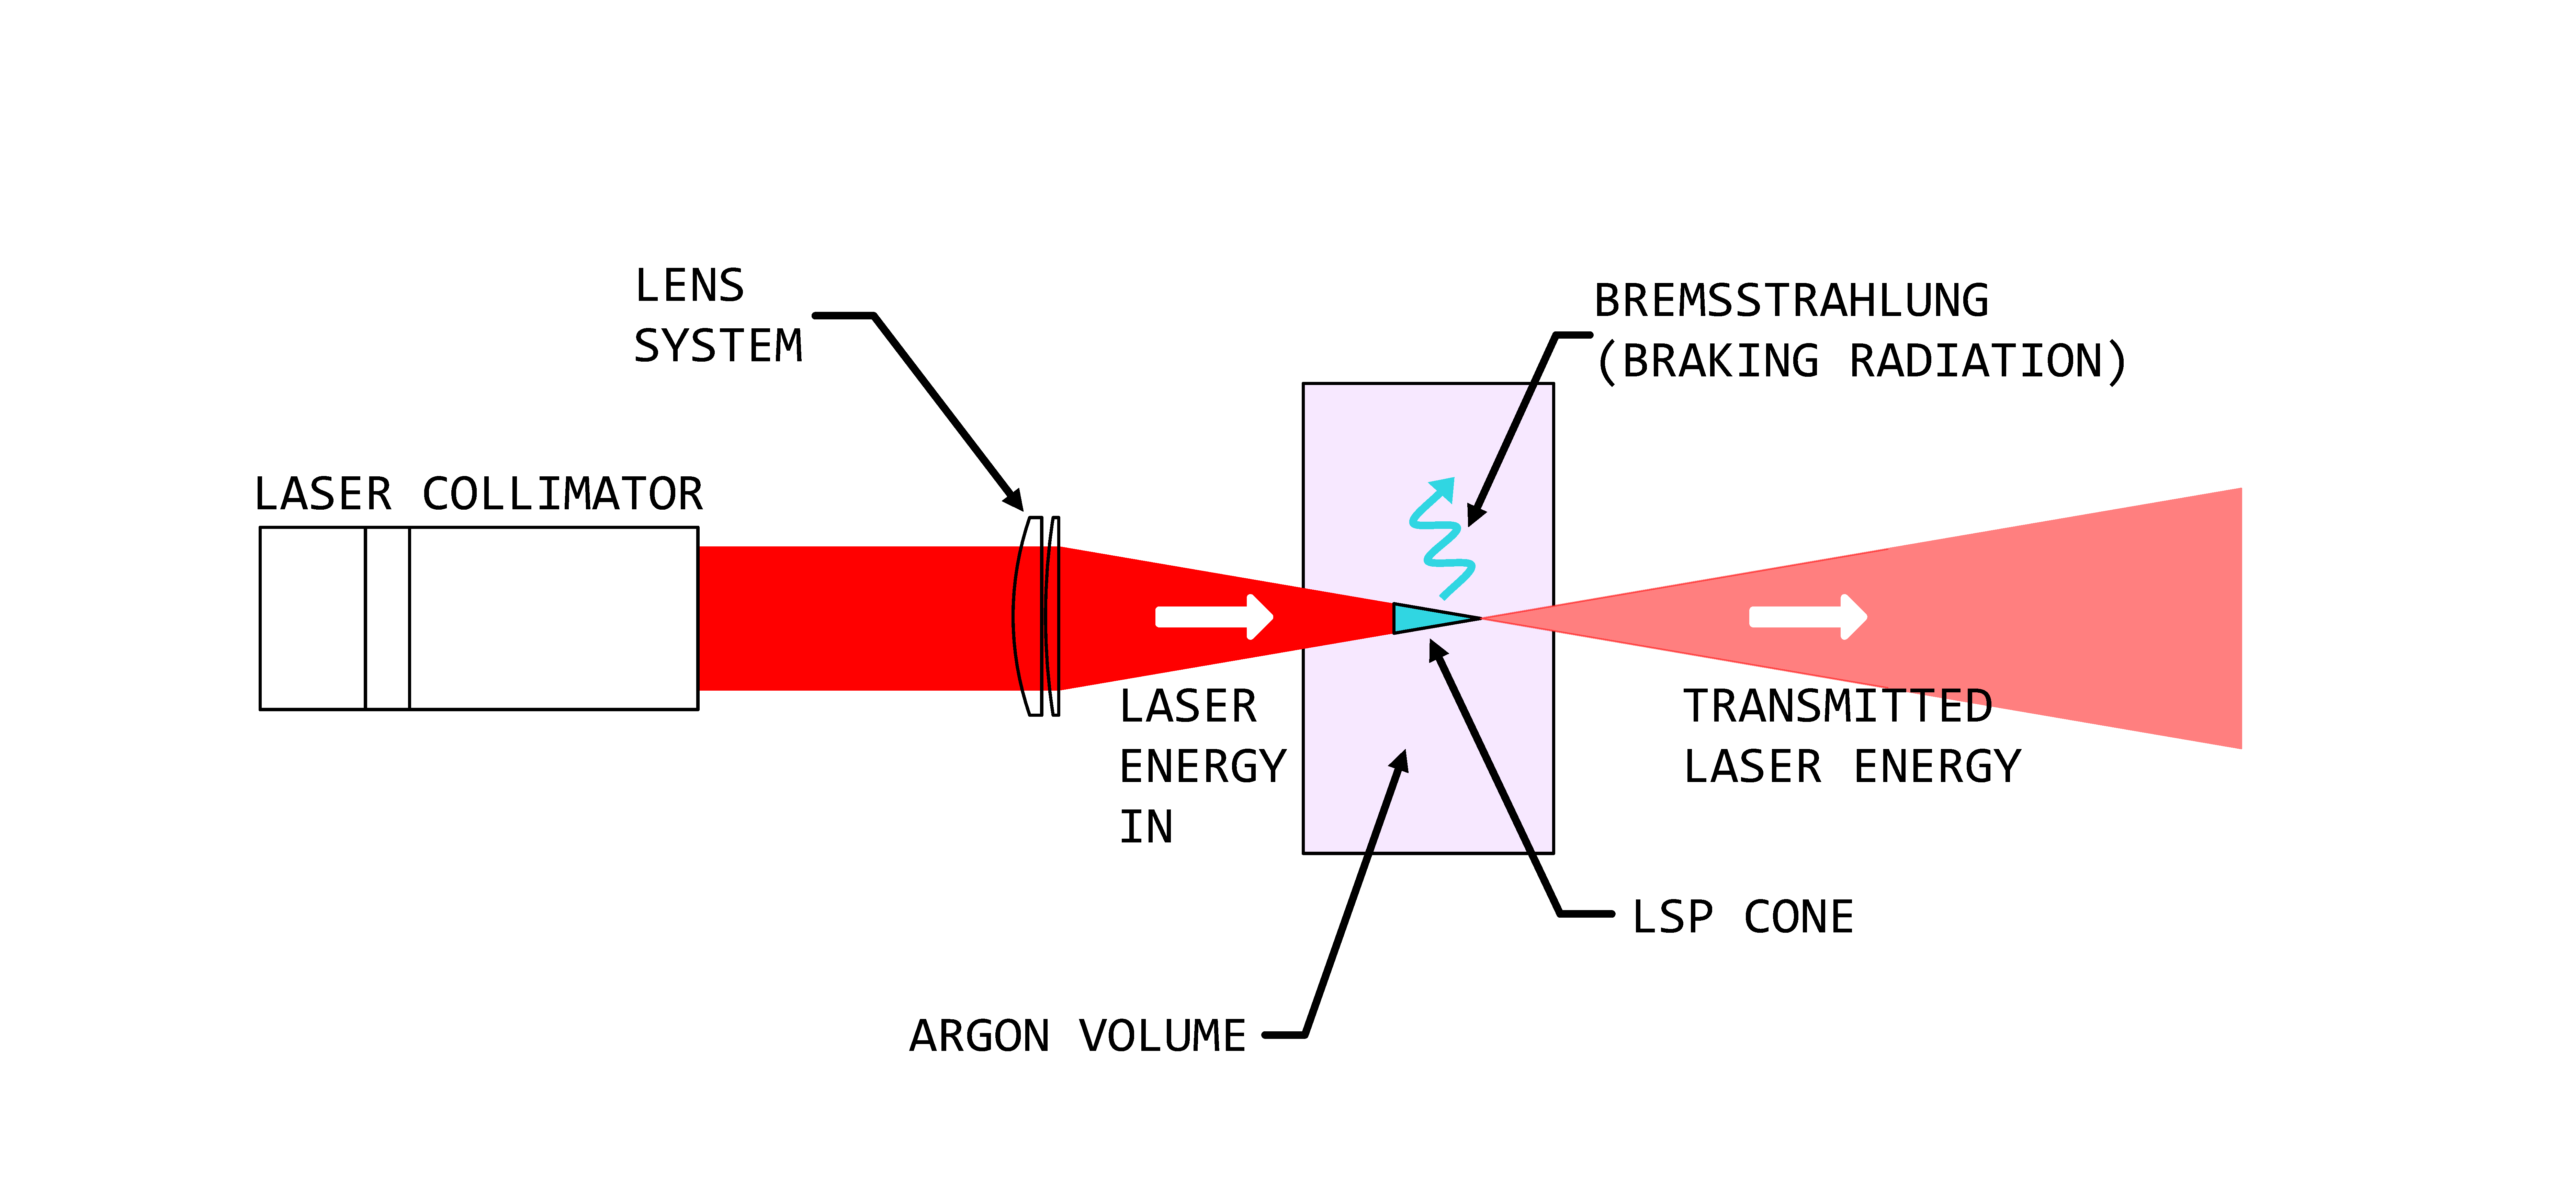
\includegraphics[width=0.85\textwidth]{assets/2 models/Modeling figure.pdf}
            \caption{0D model of an LSP inside a volume of pressurized argon}
            \label{fig:0D model}
        \end{figure}

        The calculation procedure is as follows:

        \begin{enumerate}
            \item The volume and the mass of a cone of pure argon is found at the initial temperature (\qty{300}{K}) and pressure (\qty{20}{bar})
            \item Energy from the laser pulse is added to the cone at constant pressure and the new temperature at this step is found ($T_2$)
            \item The new volume of the cone ($V_2$) is found
            \item The pressure increase in the chamber due to the expansion of the gas in the plasma cone is calculated
            \item 
          \end{enumerate}

    \section{Model results}